%\section{Foraging 2AFC}
\section{Confidence in a value guided 2AFC}
\label{task:lauglim}

\textbf{Confidence reporting and counterfactual action value updating on a trial based, 2AFC foraging task}

\subsection{Task description}
In this 2AFC, rats initiate a trial by nose-poking at a centrally located initiation port.
If they hold fixation for a minimum delay (0.2-0.4s, random uniform), the two lateral choice ports are illuminated, indicating a choice can be made.
A choice is reinforced with a drop of water after a pre-reward delay (either fixed or exponentially distributed in different task variants) if that port was baited for reward at the beginning of that trial.

At the end of each trial: \\
- an unchosen port that was not baited for reward becomes baited with probability $p$; \\
- an unchosen port that was baited for reward remains baited on the upcoming trial; \\
- a chosen port becomes baited for the upcoming trial with probability $p$.\footnote{A chosen port is known to be unbaited at the end of the trial: either it has been verified to be unbaited (unrewarded trials) or it has been made unbaited by collection of the available reward (rewarded trials). As such, it becomes baited with probability $p$ for the upcoming trial.}\\

Different values of $p$ were used, typically $p \in \{0.40, 0.05\}$ for a given session.
Different values of $p$ were associated with the two choice ports within a given block of trials, with reversals taking place at block transitions.
Blocks were typically about 100-trials long.

\subsection{Two plausible strategies}
\subsubsection{Model-free RL}
In the absence of a guiding stimulus, it is plausible that animals will simply tend to repeat choices that have been rewarded recently.
This strategy is captured by the following model:

\begin{algorithm}
\caption{Model-free RL with forgetting}
\begin{algorithmic} 
%\REQUIRE $n \geq 0 \vee x \neq 0$
%\ENSURE $y = x^n$
\FOR{$a \in \{\text{left}, \text{right}\}$}
\STATE $Q(a) \leftarrow 0$
\ENDFOR
\WHILE{$n < N$}
\STATE choice$_n$ = softmax(Q(left),Q(right))
\STATE Q(chosen) \leftarrow Q(chosen) + $\eta$ [ Reward - Q(chosen) ]
\STATE Q(unchosen) \leftarrow $\phi$ Q(unchosen)
\ENDWHILE
\end{algorithmic}
\label{alg:mf}
\end{algorithm}
with $\eta, \phi \in [0,1]$.

\begin{figure}[h!]
    \centering
    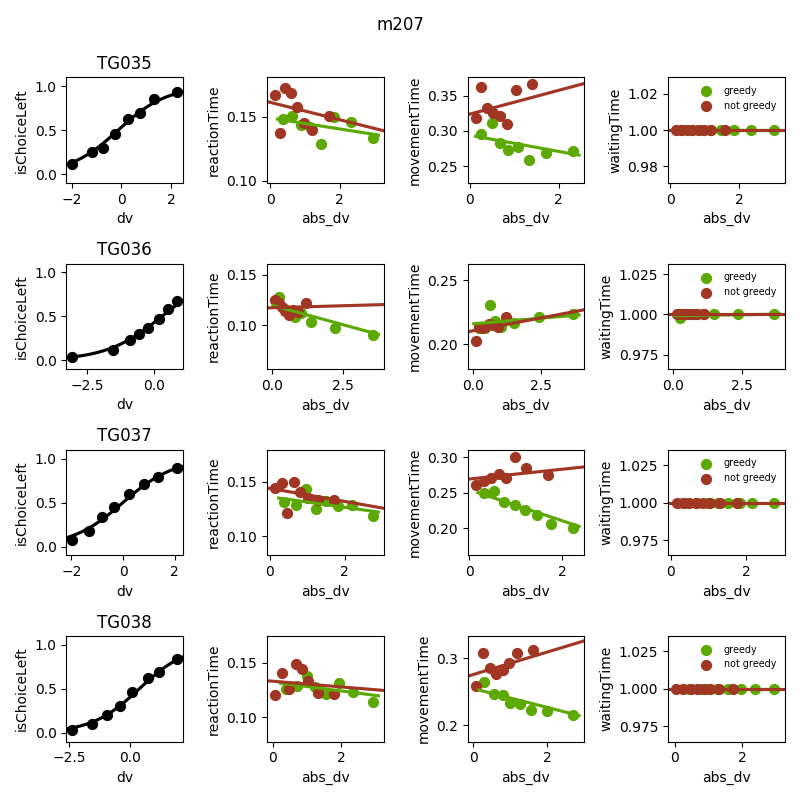
\includegraphics[width=.8\linewidth]{lauglim/dv_matching_cdda2c5_m207.png}
    \caption{\textbf{Model-free RL with forgetting, fixed reward delay}. Model captures choice behavior and movement time differences.}
    \label{fig:cdda2c5_m207}
\end{figure}

\begin{figure}[h!]
    \centering
    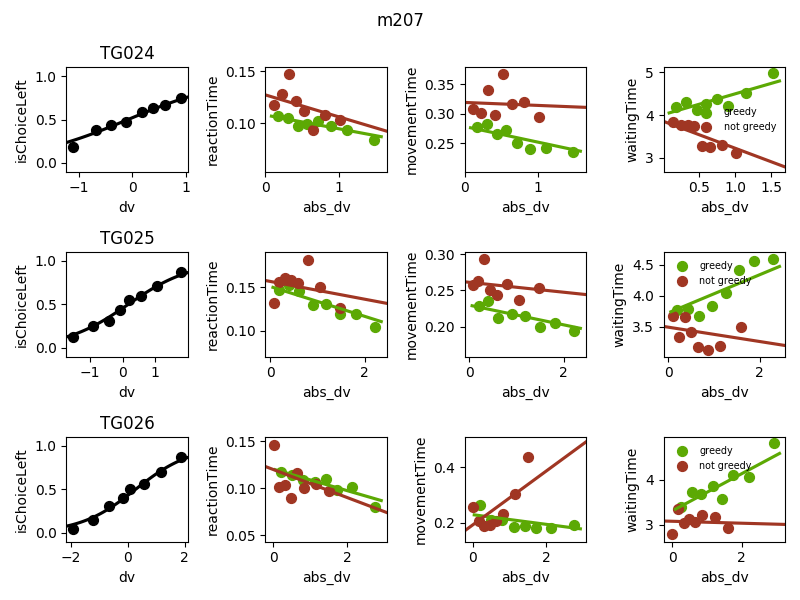
\includegraphics[width=.8\linewidth]{lauglim/dv_matching_conf_m207.png}
    \caption{\textbf{Model-free RL with forgetting, exponential reward delay}. Model captures waiting time differences.}
    \label{fig:cdda2c5_m207}
\end{figure}

\clearpage
\subsubsection{Optimal behavior} 

The reward maximizing strategy consists of always choosing the option of highest reward probability.
What is the reward probability at port $i$ after $k$ trials since it was last chosen? \\
If  $p_{i}$ is the probability that unbaited port $i$ becomes baited at each new trial, then the probability that it will remain unbaited is $1-p_i$.
The probability that it remains unbaited after $k$ trials is $\prod_{n=1}^k (1-p_i)$, and its complement is the probability that it has become baited.
In other words, the reward probability at port $i$ after $k$ trials is
\begin{align}
    P_i(R \mid k)& = 1 - \prod_{n=1}^k( 1-p_i)  \nonumber \\
    &= 1 - (1-p_i)^k    \label{eq:idobs}
\end{align}

\subsubsection*{Learning $p_i$}
The quantity $p_i$ controls when rewards are made available, but this variable is not cued in any way and must be learned by the agent.

In analogy with reinforcement learning \cite[section 9.3]{sutton2018reinforcement}, $p_i$ can be learned by minimizing the cross-entropy between $P_i(R \mid k)$ (equation \ref{eq:idobs}) and observed rewards using stochastic gradient descent.
Specifically, $p_i$ is expressed in terms of its logit transform $\pi_i = log(p_i/(1-p_i))$, and equation \ref{eq:idobs} is rewritten as
\begin{equation}
    P_i(R \mid k) = 1 - (1+e^{\pi_i})^{-k}
    \label{eq:idobs_pi}
\end{equation}.

The cross-entropy for each reward observation $r \in \{0,1\}$ is
\begin{equation}
    -J(\pi) = r \log \left(1-(1+e^\pi)^{-k}\right) + (1-r) \log \left((1+e^\pi)^{-k}\right)
    \label{eq:loss_xH}
\end{equation}

The quantity $\pi$ is then updated after each reward observation as $\pi \xleftarrow{} \pi + \eta \delta$ where $\eta$ is a step-size parameter (learning rate) and 
\begin{align}
    \delta &= - \frac{\partial J(\pi)}{\partial \pi} \nonumber \\
    &= - \frac{k e^{\pi}}{1+e^{\pi}} \left[r \left( \frac{1}{1-(1+e^\pi)^k}\right) + (1-r)  \right] \label{eq:dj_dpi}
\end{align}j.

The models fitted to the data and shown in figures \ref{fig:cdda2c5_m212} and \ref{fig:cdda2c5_m212_conf} have as free parameters the learning rate $\eta$ and the initial value of $\pi$.


\begin{figure}[h!]
    \centering
    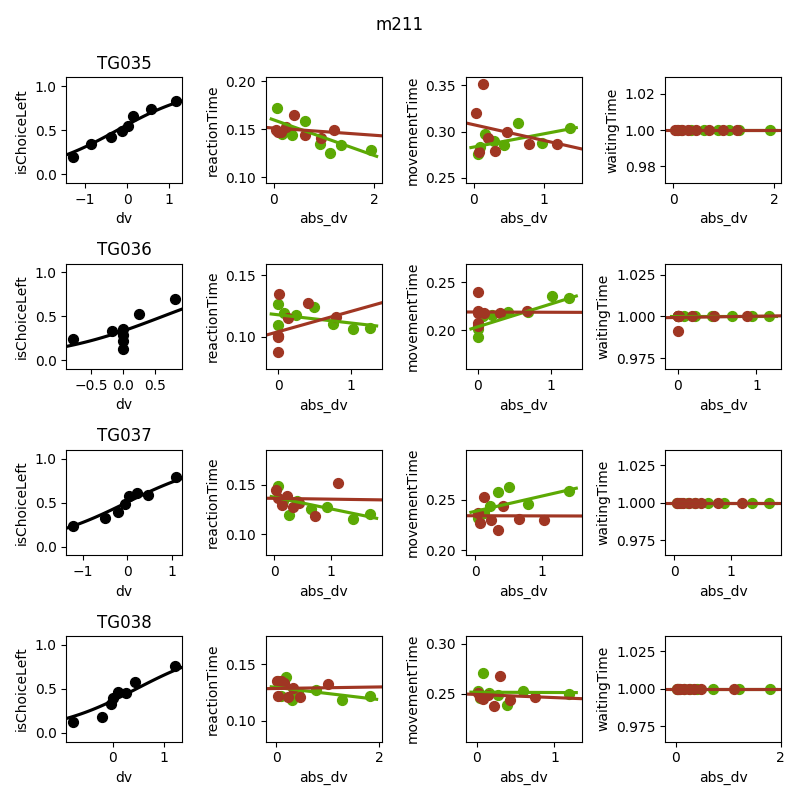
\includegraphics[width=.8\linewidth]{lauglim/dv_matching_cdda2c5_m211.png}
    \caption{\textbf{Optimal-behavior model, fixed reward delay}. Model captures choice behavior and movement time differences.}
    \label{fig:cdda2c5_m212}
\end{figure}

\begin{figure}[h!]
    \centering
    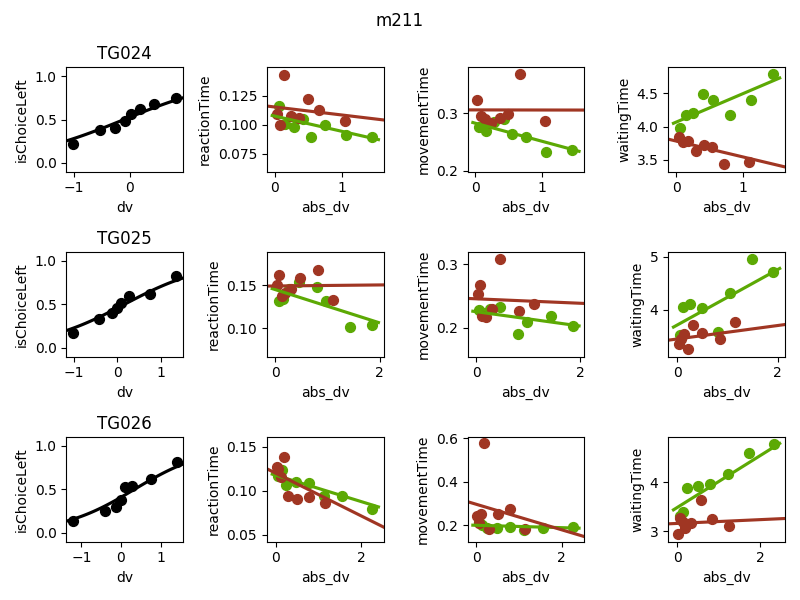
\includegraphics[width=.8\linewidth]{lauglim/dv_matching_conf_m211.png}
    \caption{\textbf{Optimal-behavior, exponential reward delay}. Model captures waiting time differences.}
    \label{fig:cdda2c5_m212_conf}
\end{figure}

\subsubsection*{To do}
Analyze trials in which predictions from RL and optimal-behavior (ideal observer) and in contradiction.

I have a mixture model thta fits choices with a weighted sum of decision variables from both these models shown here. Look at those weights.

%\subsection{Time investment}


%\subsection{Choice is well predicted from recent trial history}


%\subsection{Confidence reporting of value based decisions}


%\subsection{Updating value of action not chosen}

%\subsubsection*{Optimal behavior}


%\subsection{Models - idobs vs sarsa}

%\begin{table}[h]
%    \begin{center}
%    \begin{tabular}{l l l l}
%        {} & $p \in \mathbb{R}^L$ & $p \in \mathbb{R}^S$ & Model \\
%        \hline
%        2  & $a_{\eta}, b_{\eta}$ & $ \eta$  & $\eta \sim \text{Beta}( a_{\eta}, b_{\eta})$ \\
%        4  & $\eta$ & & $\eta \sim \text{Unif}(0,1)$ \\
%        8  & $a_{\eta}, b_{\eta}, c_\beta$ & $\eta  , \beta$  & $\eta \sim \text{Beta}( a_{\eta}, b_{\eta})$ \\
%        & & & $\beta \sim  \text{Cauchy}(0,c_\beta)$ \\
%        10 &   $a_\eta, b_\eta, \mu_{\pi_0}, \sigma_{\pi_0}$ & $\eta, \pi_0$ & $\eta \sim \text{Gamma}(a_\eta,b_\eta)$ \\
%        & & & $\pi_0 \sim \text{Gaussian}(\mu_{\pi_0}, \sigma_{\pi_0})$ \\
%        \hline
%    \end{tabular}
%    \caption[Table caption text]{Ideal observer model variants}
%    \label{table:tab_params_idobs}
%    \end{center}
%\end{table}

%\begin{table}[h]
%    \begin{center}
%    \begin{tabular}{l l l l}
%        {} & $p \in \mathbb{R}^L$ & $p \in \mathbb{R}^S$ & Model \\
%        \hline
%        3  & $\alpha, \phi, \beta$  &  & $\alpha \sim \text{Unif}(0,1)$\\
%        & & & $\phi \sim \text{Unif}(0,1)$\\
%        & & & $\beta \sim \text{Cauchy}(0,5)$ \\
%        5  & $\alpha, \phi$ & & $ \alpha \sim \text{Unif}(0,1)$ \\
%        & & & $\phi \sim \text{Unif}(0,1)$ \\
%        6  & $ \alpha, \beta$ & & $\alpha \sim \text{Unif}(0,1)$ \\
%        & & & $ \beta \sim \text{Cauchy}(0,50)$ \\
%        7  & $ a_\alpha, b_\alpha, a_\phi, b_\phi, c_\beta$ & $ \alpha, \phi, \beta$ & $ \alpha \sim \text{Beta}(a_\alpha, b_\alpha)$ \\
%        & & & $ \phi \sim \text{Beta}(a_\phi, b_\phi)$ \\
%        & & & $\beta \sim \text{Cauchy}(0,c_\beta)$ \\
%        9  & $\alpha$ & & $ \alpha \sim \text{Unif}(0,1)$ \\
%        \hline
%    \end{tabular}
%    \caption{SARSA model variants}
%    \label{table:tab_params_sarsa}
%    \end{center}
%\end{table}

%\subsection{Counterfactual action updating}


%\subsection*{Ideas and to-dos}
%JP:
%- Split trials in psyc plot between lean and rich
%- Neurons reflecting strategy II

%Behavior in bandit task with independent trials, similar reward probabilities
